%Master File:lectures.tex

\lesson{Use Heaps!}

\vspace*{-1cm}
\begin{center}
  \includegraphics[height=10cm]{heap}
\end{center}

\keywords{Heaps, Priority queues, Heap Sort, Other heaps}

%%%%%%%%%%%%%%%%%%%%%%% Next Slide %%%%%%%%%%%%%%%%%%%%%%%
\renewcommand{\Outline}{%
\begin{slide}
\section{Outline}

\begin{minipage}{10cm}
  \vfill
  \begin{enumerate}
    \outlineitem{Heaps}{heaps}
    \outlineitem{Priority Queues}{pq}
    \begin{itemize}
    \item \toplink{implHeap}{Array Implementation}
    \end{itemize}
    \outlineitem{Heap Sort}{heapSort}
    \outlineitem{Other Heaps}{otherheaps}
  \end{enumerate}
  \vfill
\end{minipage}\hfill
\begin{minipage}{14cm}
  \includegraphics[width=14cm]{heap}
\end{minipage}
\end{slide}
\addtocounter{outlineitem}{1}
}

\setcounter{outlineitem}{1}
\Outline
\toptarget{firstoutline}
%%%%%%%%%%%%%%%%%%%%%%% Next Slide %%%%%%%%%%%%%%%%%%%%%%%

\begin{slide}
\section[-2]{Heaps}

\begin{PauseHighLight}
  \begin{itemize}
  \item A (min-)heap is (from one perspective) a binary tree\pause
  \item It is a binary tree satisfying two constraints\pause
    \begin{itemize}
    \item It is a \emph{complete} tree\pause
    \item Each child has a value `greater than or equal to' its
    parent\pause
    \end{itemize}
    \begin{center}
      \includegraphics[width=0.8\linewidth]{aheap}\pause
    \end{center}
  \item \emph{complete} means that every level is fully occupied above
    the lowest level and the nodes on the lowest level are all to the
    left\pause
  \end{itemize}
\end{PauseHighLight}
\end{slide}


%%%%%%%%%%%%%%%%%%%%%%% Next Slide %%%%%%%%%%%%%%%%%%%%%%%
\Outline % Priority Queue
%%%%%%%%%%%%%%%%%%%%%%% Next Slide %%%%%%%%%%%%%%%%%%%%%%%

\begin{slide}
\section[-1]{Priority Queues}

\begin{PauseHighLight}
  \begin{itemize}
  \item One of the prime uses of heaps is to implement a priority
    queue\pause
  \item A Priority Queue is a queue with priorities\pause
  \item That is, we assign a priority to each element we add\pause
  \item The head of the queue is the element with highest priority
    (smallest number)\pause
  \item Used, for example, in simulating real time events\pause
  \item Used to implement ``greedy algorithms''\pause
  \end{itemize}
\end{PauseHighLight}
\end{slide}

%%%%%%%%%%%%%%%%%%%%%%% Next Slide %%%%%%%%%%%%%%%%%%%%%%%

\begin{slide}
\section{Priority Queue}

\begin{PauseHighLight}
  \begin{itemize}
  \item A simple Priority Queue might include
    \begin{itemize}
    \item \texttt{unsigned size()} returning the the number of
      elements
    \item \texttt{bool empty()} returns true if empty\pause
    \item \texttt{void push(T element, int priority)} adds an element\pause
    \item \texttt{T top()} returns head of queue\pause
    \item \texttt{void pop()} dequeues head of queue\pause
    \end{itemize}
  \end{itemize}
\end{PauseHighLight}

\end{slide}




%%%%%%%%%%%%%%%%%%%%%%% Next Slide %%%%%%%%%%%%%%%%%%%%%%%

\begin{slide}
\section[-2]{Array Implementation of Heaps}

\pb
\begin{itemize}
\item Because the tree is complete we can implemented the heap
  efficiently using an array\pause
\end{itemize}
\begin{center}
  \multipdf[width=0.8\textwidth]{heap_array}\pause
\end{center}

\end{slide}


%%%%%%%%%%%%%%%%%%%%%%% Next Slide %%%%%%%%%%%%%%%%%%%%%%%

\begin{slide}
\section[-2]{Code for a Priority Queue}
\toptarget{implHeap}

\begin{cpp}
#include <vector>
using namespace std;

template <typename T, typename P>
class heapPQ {
private:
  vector<pair<T, P> > array;$\pause$

public:
  
  heapPQ(unsigned capacity=11) {
    array.reserve(capacity);
  }$\pause$

  unsigned size() {return array.size();}

  bool empty() {return array.empty();}$\pause$

  const T& top() {return array[0].first;}$\pause$
\end{cpp}

\end{slide}

%%%%%%%%%%%%%%%%%%%%%%% Next Slide %%%%%%%%%%%%%%%%%%%%%%%

\begin{slide}
\section{Adding an Element}
\pb\pause\pauselevel{=1}

\begin{center}
  \multipdf[width=0.8\textwidth]{heap_push}\pause
\end{center}

\end{slide}


%%%%%%%%%%%%%%%%%%%%%%% Next Slide %%%%%%%%%%%%%%%%%%%%%%%

\begin{slide}
\section{Adding an Element}

\begin{PauseHighLight}
  \begin{cpp}
  void push(T value, P priority) {
    pair<T,P> tmp(value, priority);
    array.push_back(tmp);
    unsigned child = size() - 1;$\pause$
    
    /* Percolate Up */
    while(child!=0) {$\pause$
      unsigned parent = (child-1)>>1;  // floor((child-1)/2)$\pause$
      if (array[parent].second < array[child].second)
        return;$\pause$
      array[child] = array[parent];
      array[parent] = tmp;
      child = parent;
    }
  }$\pause$
\end{cpp}
\end{PauseHighLight}

\end{slide}

%%%%%%%%%%%%%%%%%%%%%%% Next Slide %%%%%%%%%%%%%%%%%%%%%%%

\begin{slide}
\section{Popping the Top}
\pb\pause\pauselevel{=1}

\begin{center}
  \multipdf[width=0.8\textwidth]{heap_pop}\pause
\end{center}

\end{slide}


%%%%%%%%%%%%%%%%%%%%%%% Next Slide %%%%%%%%%%%%%%%%%%%%%%%

\begin{slide}
\section{Popping the Top}

\begin{cpp}
    void pop() {
    unsigned parent = 0;
    pair<T, P> tmp = array.back();
    array[0] = tmp;
    array.pop_back();$\pause$
    unsigned child = 1;

    /* Percolate down */
    while(child<size()) {$\pause$
      if (child+1<=size() && array[child+1].second < array[child].second)
	++child;$\pause$
      if (array[child].second > array[parent].second)
	return;$\pause$
      array[parent] = array[child];
      array[child] = tmp;
      parent = child;
      child = 2*parent + 1;
    }
  }$\pause$
\end{cpp}
\end{slide}

%%%%%%%%%%%%%%%%%%%%%%% Next Slide %%%%%%%%%%%%%%%%%%%%%%%

\begin{slide}
\section[-1]{Heaps in Action}
\pb\pause\pauselevel{=1}
\begin{center}
  \multipdf[width=0.9\textwidth]{heaps_in_action}\pause
\end{center}


\end{slide}
%%%%%%%%%%%%%%%%%%%%%%% Next Slide %%%%%%%%%%%%%%%%%%%%%%%

\begin{slide}
\section{Time Complexity of Heaps}

\begin{PauseHighLight}
  \begin{itemize}
  \item The two important operation are \texttt{add} and
    \texttt{removeMin}\pause
  \item These both either percolating an element up the tree or
    percolating an element down the tree\pause
  \item The number of operations depends on the depth of the tree which
    is $\Theta(\log(n))$\pause
  \item Thus \texttt{add} and \texttt{removeMin} are $O(\log(n))$\pause
  \item Except \texttt{add} could also require resizing the
  array\pause\nhl{,} but the amortised cost of this is low\pause
  \end{itemize}
\end{PauseHighLight}

\end{slide}



%%%%%%%%%%%%%%%%%%%%%%% Next Slide %%%%%%%%%%%%%%%%%%%%%%%

\begin{slide}
\section[-1]{Real Time Simulation}

\begin{PauseHighLight}
  \begin{itemize}
  \item A nice application of priority queues is to perform real time
    simulations\pause
  \item I was once modelling a neural network where neuron fired an
    impulse which would then be received by other neurons\pause
    \begin{center}
      \includegraphics[width=0.5\linewidth]{neuralNet}
    \end{center}
  \end{itemize}
\end{PauseHighLight}

\end{slide}

%%%%%%%%%%%%%%%%%%%%%%% Next Slide %%%%%%%%%%%%%%%%%%%%%%%

\begin{slide}
\section{Synchronised Firing}

\begin{PauseHighLight}
  \begin{itemize}
  \item We wanted to show that if a group of neurons fired together they
    could make another group of neurons fire in synchrony despite the
    fact that it would take different times for the receiving neurons to
    feel the pulse (due to the different lengths of the axons)\pause
  \item A famous Israeli group had ``proved'' this couldn't happen\pause
  \item Using a priority queue we modelled the neurons
    \begin{itemize}
    \item When a neuron fired the receiving neurons would be put on a
      priority queue according to when they received the pulse\pause
    \item If the receiving neurons received enough pulse in a short
      enough time they would then fire\pause
    \end{itemize}
  \end{itemize}
\end{PauseHighLight}

\end{slide}

%%%%%%%%%%%%%%%%%%%%%%% Next Slide %%%%%%%%%%%%%%%%%%%%%%%

\begin{slide}
\section{Efficient Modelling}

\begin{PauseHighLight}
  \begin{itemize}
  \item Using a priority queue meant we knew when the next event would
    happen\pause
  \item We did not have to run a clock where most of the time nothing
    happened\pause
  \item This allowed us to perform a very large simulation efficiently\pause
  \item The simulation showed that the pulse of neurons synchronised
    despite the ``proof'' that this wouldn't happen\pause
  \end{itemize}
\end{PauseHighLight}

\end{slide}


%%%%%%%%%%%%%%%%%%%%%%% Next Slide %%%%%%%%%%%%%%%%%%%%%%%
\Outline % Heap Sort
%%%%%%%%%%%%%%%%%%%%%%% Next Slide %%%%%%%%%%%%%%%%%%%%%%%

\begin{slide}
\section[-2]{Heap Sort}

\begin{PauseHighLight}
  \begin{itemize}
  \item A priority queue suggests a very simple way of performing
    sort\pause
  \item We simply add elements to a heap and then take them off
  again
  \begin{java}
    template <typename T>
    void sort(vector<T> aList)
    {
        HeapPQ<T> aHeap = new HeapPQ<T>(aList.size());$\pause$
        for (T element: aList)
          aHeap.push(element, element);$\pause$

        aList.clear();$\pause$
        while(aHeap.size() > 0) {
          aList.push_back(aHeap.top());
          aHeap.pop();
        }
    }$\pause$
  \end{java}
  \item Note that this is not an in-place sort algorithm (i.e. it uses
    lots of memory)\pause
  \end{itemize}
\end{PauseHighLight}

\end{slide}

%%%%%%%%%%%%%%%%%%%%%%% Next Slide %%%%%%%%%%%%%%%%%%%%%%%

\begin{slide}
\section{Example of Heap Sort}
\pb\pause\pauselevel{=1}
\begin{center}
  \multipdf[width=\textwidth]{heapSort}\pause
\end{center}


\end{slide}


%%%%%%%%%%%%%%%%%%%%%%% Next Slide %%%%%%%%%%%%%%%%%%%%%%%

\begin{slide}
\section[-2]{Complexity of Heap Sort}

\begin{PauseHighLight}
  \begin{itemize}
  \item As we have to add $n$ elements and then remove $n$ elements the
    time complexity is log-linear, i.e. $O(n\,\log(n))$\pause\vspace*{-1cm}
    \begin{center}
      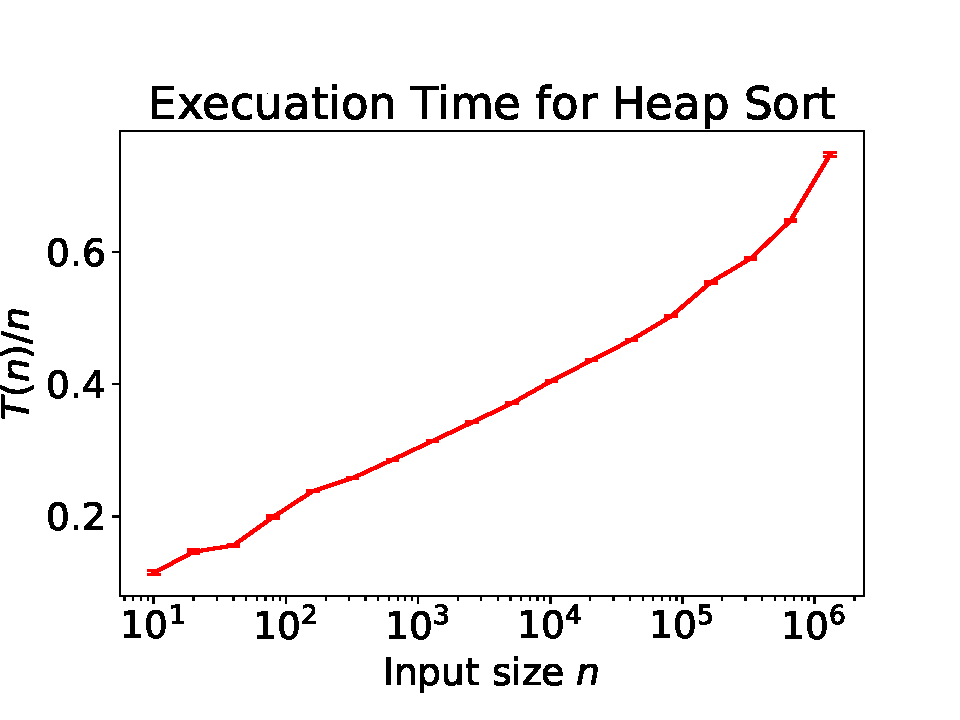
\includegraphics[height=12cm]{heapSortTimings}\pause
    \end{center}\vspace*{-1cm}
  \item This is actually a very efficient algorithm\pause
  \end{itemize}
\end{PauseHighLight}

\end{slide}


%%%%%%%%%%%%%%%%%%%%%%% Next Slide %%%%%%%%%%%%%%%%%%%%%%%
\Outline % Other Heaps
%%%%%%%%%%%%%%%%%%%%%%% Next Slide %%%%%%%%%%%%%%%%%%%%%%%

\begin{slide}
\section{Other Heaps}

\begin{PauseHighLight}
  \begin{itemize}
  \item Binary Heaps are so useful that other types of heaps have been
    developed\pause
  \item The simplest enhancement is to combine a binary heap with a map
    which maintains a pointer to each element\pause
  \item The map has to be updated every time elements are moved in the
    heap (fortunately only $O(\log(n))$ elements are move each time the
    heap is updated)\pause
  \item The advantage of this heap is that the priorities of elements
    can be changed (involving percolating elements up or down the tree)\pause
  \end{itemize}
\end{PauseHighLight}


\end{slide}


%%%%%%%%%%%%%%%%%%%%%%% Next Slide %%%%%%%%%%%%%%%%%%%%%%%

\begin{slide}
\section{Merging Heaps}

\begin{PauseHighLight}
  \begin{itemize}
  \item One common demand on a heaps is to merge two heaps\pause
  \item Unfortunately binary heaps are not efficiently merged\pause
  \item There are a variety of different heaps (leftist heaps, skew
    heaps, binomial queues, \ldots) designed to be merged\pause
  \item All these heaps are real binary trees (i.e. represented by
    pointers rather than put in an array)\pause
  \item They are slower than a binary heap because indexing is slightly
    slower as is creating node objects\pause
  \item However, they allow merging\pause
  \end{itemize}
\end{PauseHighLight}

\end{slide}

%%%%%%%%%%%%%%%%%%%%%%% Next Slide %%%%%%%%%%%%%%%%%%%%%%%

\begin{slide}
\section{Other Operations}

\begin{PauseHighLight}
  \begin{itemize}
  \item All other operations are achieved by merging
    \begin{itemize}
    \item Adding an element is achieved by merging the current heap with
      a heap of one element\pause
    \item Removing the minimum element is achieved by removing the root
      and merging the left and right tree\pause
    \end{itemize}
  \item For details see the course text (you won't be examined on the
    details of these heaps)\pause
  \end{itemize}
\end{PauseHighLight}


\end{slide}




%%%%%%%%%%%%%%%%%%%%%%% Next Slide %%%%%%%%%%%%%%%%%%%%%%%

\begin{slide}
\section[-1]{Lessons}

\begin{PauseHighLight}
  \begin{itemize}
  \item Heaps are a powerful data structure---they are particularly
    useful for implementing priority queues\pause
  \item Heaps are binary trees that can be implemented as arrays\pause
  \item Priority queue have many (often surprising uses)\pause
    \begin{itemize}
    \item They are used when you need a queue with priorities, e.g. in
      operating systems\pause
    \item They can be used to perform pretty efficient sort\pause
    \item They are often used for implementing greedy type
      algorithms\pause
    \item One important application is in real time simulations\pause
    \end{itemize}
  \item There exists many extensions of heaps\pause
  \end{itemize}
\end{PauseHighLight}

\end{slide}

